\section{QMA complexity of approximate counting}

\label{sec:SBPQMA}

This section establishes
an 
optimal lower bound on the $\mathsf{QMA}$
complexity of approximate counting.
We first lower bound the $\mathsf{SBQP}$ complexity
of the $\mathsf{AND}_2 \circ \mathsf{ApxCount}_{N,w}$ problem (
\Cref{thm:sbqp}). 
This implies a $\mathsf{QMA}$ lower bound
for $\mathsf{ApxCount}_{N,w}$ via \Cref{lem:guessing},
but it is not quantitatively optimal. 
We prove the optimal $\mathsf{QMA}$ lower bound 
(\Cref{thm:qmabound}) via
\Cref{lem:betterforqma}, which
leverages additional properties 
of 
the $\mathsf{SBQP}$ protocol derived via
\Cref{lem:guessing}
from any $\mathsf{QMA}$ protocol with small
witness length. Finally, \Cref{cor:qma_separation}
describes new oracle separations that
are immediate consequences of \Cref{thm:qmabound} and \Cref{thm:sbqp}. 

%
\subsection{Lower bound for \texorpdfstring{$\mathsf{SBQP}$}{SBQP} algorithms}
\label{sec:SBQP} 

Our lower bound on the $\cl{SBQP}$ complexity of $\AndApxCount$ hinges 
on the following theorem. \ The theorem
uses Laurent polynomials to prove a degree lower bound for bivariate
polynomials that satisfy an upper bound on an \textquotedblleft
L\textquotedblright -shaped pair of rectangles and a lower bound at a nearby
point:

\begin{theorem}
\label{thm:L} Let $0<w<32w<N$ and $M\geq 1$. \ Let $R_{1}=[4w,N]\times \lbrack 0,w/2]$ and
$R_{2}=[0,w/2]\times \lbrack 4w,N]$ be disjoint rectangles in the plane, and
let $L=R_{1}\cup R_{2}$. \ Let $p(x,y)$ be a real polynomial of degree $d$
with the following properties:
\begin{enumerate}
\item $p(4w, 4w) \ge 1.5 \cdot M$.
\item $0 \le p(x, y) \le 1$ for all $(x, y) \in L$.
\end{enumerate}
Then $d = \Omega(\sqrt{N/w} \cdot \log M)$.
\end{theorem}

\begin{figure}[tbp]
\centering
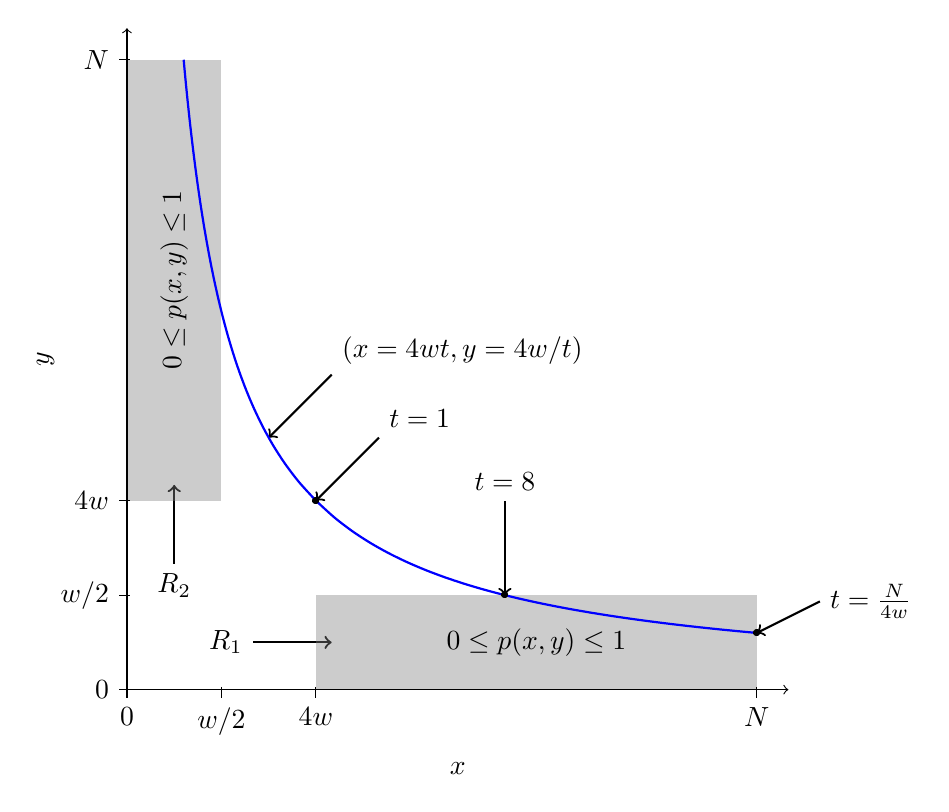
\begin{tikzpicture}[y=0.4cm, x=0.4cm]
	\pgfmathsetmacro{\N}{20}
	\pgfmathsetmacro{\w}{3}
	\pgfmathsetmacro{\tw}{\w+\w}
	\pgfmathsetmacro{\Np}{\N+1}

%
	\draw[<-,thick] (\tw+0.5, \w/2) -- (\w+1,\w/2) node[anchor=east] {$R_1$};
	\draw[<-,thick] (\w/2, \tw+0.5) -- (\w/2,\w+1) node[anchor=north] {$R_2$};

%
	\fill[gray,opacity=.4] (\tw,0) -- (\tw,\w) -- (\N,\w) -- (\N,0);
	\fill[gray,opacity=.4] (0,\tw) -- (\w,\tw) -- (\w,\N) -- (0,\N);

%
	\draw[->] (0,0) -- coordinate (x axis mid) (\Np,0);
    	\draw[->] (0,0) -- coordinate (y axis mid) (0,\Np);
    	
%
	\draw[<-,thick] (\tw,\tw) -- (\tw+2,\tw+2) node[anchor=south west] {$t=1$};   	
	\draw[<-,thick] (\w*4,\w) -- (\w*4,\w*2) node[anchor=south] {$t=8$};
	\draw[<-,thick] (\N,4*\w*\w/\N) -- (\N+2,1+4*\w*\w/\N) node[anchor=west] {$t=\frac{N}{4w}$};
	\draw[<-,thick] (1.5*\w,2*\w*4/3) -- (1.5*\w+2,2*\w*4/3+2) node[anchor=south west] {$(x=4wt,y=4w/t)$};
    	
    \draw (0,1pt) -- (0,-3pt) node[anchor=north] {0};
    \draw (\w,1pt) -- (\w,-3pt) node[anchor=north] {$w/2$\vphantom{l}};
    \draw (\tw,1pt) -- (\tw,-3pt) node[anchor=north] {$4w$};
    \draw (\N,1pt) -- (\N,-3pt) node[anchor=north] {$N$};

    \draw (1pt,0) -- (-3pt,0) node[anchor=east] {0};
    \draw (1pt,\w) -- (-3pt,\w) node[anchor=east] {$w/2$};
    \draw (1pt,\tw) -- (-3pt,\tw) node[anchor=east] {$4w$};
    \draw (1pt,\N) -- (-3pt,\N) node[anchor=east] {$N$};

%
	\node[below=0.8cm] at (x axis mid) {$x$};
	\node[rotate=90, above=0.8cm] at (y axis mid) {$y$};
	\node at (\w+\N/2, \w/2) {$0 \le p(x, y) \le 1$};
	\node[rotate=90] at (\w/2, \w+\N/2) {$0 \le p(x, y) \le 1$};

     \draw[thick,domain=1:{\N/(2*\w)},smooth,variable=\t,blue] plot ({2*\w*\t},{2*\w/\t});
%
     \draw[thick,domain=1:{\N/(2*\w)},smooth,variable=\t,blue] plot ({2*\w/\t},{2*\w*\t});
     \node at ({\w+\w},{\w+\w}) {\tiny\textbullet};
     \node at (4*\w,\w) {\tiny\textbullet};
     \node at (\N,4*\w*\w/\N) {\tiny\textbullet};
\end{tikzpicture}
\caption{Diagram of \Cref{thm:L} (not drawn to scale).}
\label{fig:L}
\end{figure}

\begin{proof}
Observe that if $p(x, y)$ satisfies the statement of the theorem, then so does $p(y, x)$. This is because the constraints in the statement of the theorem are symmetric in $x$ and $y$ (in particular, because $R_1$ and $R_2$ are mirror images of one another along the line $x = y$; see \Cref{fig:L}). As a result, we may assume without loss of generality that $p$ is symmetric, i.e.,\ $p(x, y) = p(y, x)$. Else, we may replace $p$ by $\frac{p(x, y) + p(y, x)}{2}$ because the set of polynomials that satisfy the inequalities in the statement of the theorem are closed under convex combinations.

Consider the hyperbolic parametric curve $(x = 4wt, y=4w/t)$ as it passes through $R_1$ (see \Cref{fig:L}). We can view the restriction of $p(x, y)$ to this curve as a Laurent polynomial $\ell(t) = p(4wt, 4w/t)$ of positive and negative degree $d$. The bound of $p(x,y)$ on all of $R_1$ implies that $|\ell(t)| \le 1$ when $t \in [8, \frac{N}{4w}]$ and that $\ell(1) \ge 1.5$ (see \Cref{fig:L}). Moreover, the condition that $p(x, y)$ is symmetric implies that $\ell(t) = \ell(1/t)$.

By \Cref{lem:symmetric} for symmetric Laurent polynomials, $\ell(t)$ can be viewed as a degree $d$ polynomial $q(t + 1/t)$. Under the transformation $s = t + 1/t$, $q$ satisfies $|q(s)| \le 1$ for $s \in [8 + 1/8, \frac{N}{4w} + \frac{4w}{N}]$ and $q(2) \ge 1.5 M$. Note that the length of the interval $[8 + 1/8, \frac{N}{4w} + \frac{4w}{N}]$ is $\Theta(N/w)$ because $w < N$. By an appropriate affine transformation of $q$, we can conclude from \Cref{paturilem} with $\mu = \Theta(w/N)$ that $d = \Omega(\sqrt{N/w} \cdot \log M)$.
\end{proof}

Why is \Cref{thm:L} useful? \ One may be tempted to apply this theorem
directly to the polynomial $p(x,y)$ obtained in \Cref{lem:symmetrization} to
conclude a degree lower bound (and thus a query complexity lower bound), as
the \textquotedblleft L\textquotedblright -shaped pair of rectangles $
L=R_{1}\cup R_{2}$ correspond to \textquotedblleft no\textquotedblright\
instances of $\mathsf{AND}_{2}\circ \mathsf{ApxCount}_{N,w}$, while $(4w,4w)$
corresponds to a \textquotedblleft yes\textquotedblright\ instance. \
However, even though $p(x,y)$ is bounded at lattice points in $L$, it need
not be bounded along the entirety of $L$.\footnote{
One can nevertheless use this intuition to obtain a nontrivial (though
suboptimal) lower bound by inspecting $p$ alone. Using the Markov brothers'
inequality (\Cref{markovlem}), if $\deg (p)=o(\sqrt{w})$, then the bounds on
$p(x,y)$ at lattice points in $L$ imply that $|p(x,y)|\leq 1+o_{w}(1)$ for
all $(x,y)\in L$. Thus, \Cref{thm:L} applies if $\deg (p)=o(\sqrt{w})$, so
overall we get a lower bound of $\Omega \left( \min \left\{ \sqrt{w},\sqrt{
N/w}\right\} \right) $ for the $\mathsf{SBQP}$ query complexity of $\mathsf{
AND}_{2}\circ \mathsf{ApxCount}_{N,w}$. See 
\href{https://arxiv.org/abs/1902.02398}{arXiv:1902.02398} for details.} \ 

To obtain a lower bound, we
instead use the connection between the polynomials $p(x,y)$ and $q(s,t)$
from \Cref{lem:symmetrization}, and establish \Cref{thm:sbqp} from the
introduction, restated for convenience:

\sbqp*

\begin{proof}
Let $N > 32w$ (otherwise the theorem holds trivially). Since $Q$ is an $\mathsf{SBQP}$ algorithm, we may suppose that $Q$ accepts with probability at least $2\alpha$ on a ``yes'' instance and with probability at most $\alpha$ on a ``no'' instance (note that $\alpha$ may be exponentially small in $N$). Take $p(x,y)$ and $q(s, t)$ to be the symmetrized bivariate polynomials of degree at most $2T$ defined in \Cref{lem:symmetrization}. Define $L' = ([0, w] \times [0, w]) \cup ([0, w] \times [2w, N]) \cup ([2w, N] \times [0, w])$. The conditions on the acceptance probability of $Q$ for all $S_0, S_1$ that satisfy the $\ApxCount$ promise imply that $p(x, y)$ satisfies these corresponding conditions:
\begin{enumerate}
\item $1 \ge p(x, y) \ge 2\alpha$ for all $(x, y) \in \left([2w, N] \times [2w, N]\right) \cap \mathbb{Z}^2$.
\item $0 \le p(x, y) \le \alpha$ for all $(x, y) \in L' \cap \mathbb{Z}^2$.
\end{enumerate}

Our strategy is to show that if $T = o(w)$, then these conditions on $p$ imply that the polynomial $q(s, t) \cdot \frac{0.9}{\alpha}$ satisfies the statement of \Cref{thm:L} for all sufficiently large $w$. This in turn implies $T = \Omega(\sqrt{N/w})$. This allows us conclude that either $T = \Omega(w)$ or $T = \Omega(\sqrt{N/w})$, which proves the theorem.

Suppose $T = o(w)$, so that $p(x, y)$ and $q(s, t)$ both have degree $d=o(w)$. We begin by upper bounding $p(x, y)$ at the lattice points $(x, y)$ outside of $L'$. 
We claim the following:
\begin{enumerate}[(a)]
\item $|p(x, y)| \le \alpha \cdot a \cdot \exp(bd^2 / w) \le \alpha \cdot a \cdot \exp(bd)$ whenever $(x, y) \in L'$ and either $x$ or $y$ is an integer, where $a$
and $b$ are the constants from \Cref{lem:coppersmith_rivlin}. This follows from \Cref{lem:coppersmith_rivlin} by fixing either $x$ or $y$ to be an integer and viewing the resulting restriction of $p(x, y)$ as a univariate polynomial in the other variable.
\item $|p(x, y)| \le \alpha \cdot a \cdot \exp(bd) \cdot \exp(2\sqrt{3}d) = \alpha \cdot a \cdot \exp((b + 2\sqrt{3})d)$ whenever $x \in [w, 2w]$, $y \in [0, w]$, and $y$ is an integer. This follows \Cref{paturilem}: consider the univariate polynomial $p(\cdot, y)$ on the intervals $[0, w]$ and $[2w, 3w]$, where it is bounded by (a).
\item $|p(x, y)| \le \alpha \cdot a \cdot \exp((b + 2\sqrt{3})d) \cdot a \cdot \exp(bd^2/w) \le \alpha \cdot a^2 \cdot \exp((2b + 2\sqrt{3})d)$ whenever $x \in [w, 2w]$ and $y \in [0, w]$. This follows from \Cref{lem:coppersmith_rivlin}: consider the univariate polynomial $p(x, \cdot)$ on the interval $[0, w]$, where it is bounded at integer points by (b).
\item $|p(x, y)| \le \alpha \cdot a^2 \cdot \exp((2b + 2\sqrt{3})d) \cdot \exp(4dy/w) = \alpha \cdot a^2 \cdot \exp((2b + 2\sqrt{3} + 4y/w)d)$ whenever $x \in [0, N]$, $y \in [w + 1, N]$, and $x$ is an integer. This follows from  \Cref{paturilem}: consider the univariate polynomial $p(x, \cdot)$ on the interval $[0, w]$, where it is bounded by (a) when $x \in [0, w]$ or $x \in [2w, N]$, or bounded by (c) when $x \in [w, 2w]$. 
By an affine shift, this corresponds to applying \Cref{paturilem} with $\mu = 2y/w - 2$, with the observation that $\sqrt{2\mu + \mu^2} < \mu + 2$.
\end{enumerate}

We now use this to upper bound $q(s, t)$ when $s \in [4w, N]$ and $t \in [0, w/2]$. Let $X$ and $Y$ be drawn from $N$-trial binomial distributions with means $s$ and $t$, respectively,
so that $q(s, t) = \E[p(X,Y)]$. Using the above bounds and basic probability, we have 
\begin{align}
0 \leq q(s, t) = \E[p(X,Y)] &\le \alpha \cdot \bigg( \Pr[X \ge 2w, Y \le w] + \Pr[X \le 2w, Y \le w] \cdot a \cdot \exp\left(\left(b+2\sqrt{3}\right)d\right)  \nonumber \\
& \quad + \sum_{y = w+1}^N \Pr[Y = y] \cdot a^2 \cdot \exp\left(\left(2b + 2\sqrt{3} + 4y/w\right)d\right) \bigg)\\
&\le \alpha \cdot \bigg(1 + \Pr[X \le 2w] \cdot a \cdot \exp\left(\left(b+2\sqrt{3}\right)d\right)   \nonumber \\
& \quad + \sum_{y = w+1}^N \Pr[Y \ge y] \cdot a^2 \cdot \exp\left(\left(2b + 2\sqrt{3} + 4y/w\right)d\right)\bigg).
\end{align}
The probabilities above are easily bounded with a Chernoff bound:
\begin{align}
q(s, t)=\E[p(X,Y)] &\le \alpha \cdot \bigg( 1 + a \cdot \exp\left(\left(b+2\sqrt{3}\right)d - w/2\right)  \nonumber\\
& \quad + \sum_{y = w+1}^N a^2 \cdot \exp\left(\left(2b + 2\sqrt{3} + 4y/w\right)d - y/6\right)\bigg).
\end{align}
Because $a$ and $b$ are universal constants from \Cref{lem:coppersmith_rivlin}, when $d = o(w)$, the first exponential term becomes arbitrarily small for all sufficiently large $w$. Moreover, for all sufficiently large $w$, the remaining sum becomes bounded by a geometric sum. For some constant $c$, we have
\begin{align*}
\sum_{y = w+1}^N a^2 \cdot \exp\left(\left(2b + 2\sqrt{3} + 4y/w\right)d - y/6\right) &\le \sum_{y = w+1}^\infty c \cdot \exp\left(-y/12\right)\\
&\le \frac{c}{1 - \exp(-1/12)} \cdot \exp(-w/12)\\
&= o_w(1).
\end{align*}
Thus we conclude that $0 \le q(s, t) \le \alpha \cdot (1 + o_w(1))$ when $s \in [4w, N]$ and $t \in [0, w/2]$ (i.e.,\ $(s, t) \in R_1$ in the statement of \Cref{thm:L}). By symmetry, we can conclude the same bound when $s \in [0, w/2]$ and $t \in [4w, N]$ (i.e.,\ $(s, t) \in R_2$ in the statement of \Cref{thm:L}).

Now, we lower bound $q(4w, 4w)$. Let $X$ and $Y$ be drawn from independent $N$-trial binomial distributions with mean $4w$, so that $q(4w, 4w) = \mathbb{E}\left[p(X,Y)\right]$. Then we have 
\begin{align*}
\mathbb{E}\left[p(X,Y)\right] &\ge 2\alpha \cdot \Pr[X \ge 2w, Y \ge 2w]\\
&\ge 2\alpha \cdot \left(1 - \Pr[X \le 2w] - \Pr[Y \le 2w]\right)\\
&\ge 2\alpha \cdot \left(1 - 2\exp(-w/2)\right)\\
&\ge 2\alpha \cdot (1 - o_w(1))
\end{align*}
We conclude that $q(s, t) \cdot \frac{0.9}{\alpha}$ satisfies the statement of \Cref{thm:L} (with $M=1$) for all sufficiently large $w$.
\end{proof}

We remark that this lower bound is tight, i.e.,\ there exists an $\mathsf{
SBQP}$ algorithm that makes $O\left( \min \left\{ w,\sqrt{N/w}\right\}
\right) $ queries. \ The $O(\sqrt{N/w})$ upper bound follows from the $
\mathsf{BQP}$ algorithm of Brassard, H{\o }yer, and Tapp \cite{bht:count}. \
The $O(w)$ upper bound is in fact an $\mathsf{SBP}$ upper bound with the
following algorithmic interpretation: first, guess $w+1$ items randomly from
each of $S_{0}$ and $S_{1}$. \ Then, verify using the membership oracle that
the first $w+1$ items all belong to $S_{0}$ and that the latter $w+1$ items
all belong to $S_{1}$, accepting if and only if this is the case. \ Clearly,
this accepts with nonzero probability if and only if $\left\vert
S_{0}\right\vert \geq w+1$ and $\left\vert S_{1}\right\vert \geq w+1$. 

%
\subsection{Lower bound for \texorpdfstring{$\mathsf{QMA}$}{QMA}}
\label{sec:QMA} 

In this section, we establish the optimal $\mathsf{QMA}$ lower bound 
(\Cref{thm:qmabound}).
We begin by quantitatively improving the $\mathsf{SBQP}$
lower bound for $\AndApxCount$ of \Cref{thm:sbqp},
under the stronger assumption that the parameter $\alpha$ 
in the $\mathsf{SBQP}$ protocol is not smaller than $2^{-w}$.
(In addition to a stronger
conclusion, this assumption also permits a considerably simpler
analysis than was required to prove \Cref{thm:sbqp}).

\begin{lemma}
\label{lem:betterforqma}
Consider any quantum query algorithm $Q^{\mathcal{O}_{S_{0}},\mathcal{O}_{S_{1}}}$
for $\AndApxCount$
that makes $T$ queries to the membership oracles
$\mathcal{O}_{S_{0}}$ and $\mathcal{O}_{S_{1}}$
for the two instances of $\ApxCount$ and
satisfies the following. For some $m=o(w)$, $\alpha=2^{-m}$, and $M \in [1, \alpha^{-1}]$:
\begin{enumerate}
\item If $x \in L$, then $\Pr\left[Q(x) \text{ accepts}\right] \ge
\alpha$.
\item If $x \not\in L$, then $\Pr\left[Q(x) \text{ accepts}\right] \le
\alpha/(2 M)$.
\end{enumerate}
Then $T = \Omega\left(\sqrt{N/w} \cdot \log M\right)$
\end{lemma}
\begin{proof}
As in the proof of \Cref{thm:sbqp}, define $L' = ([0, w] \times [0, w]) \cup ([0, w] \times [2w, N]) \cup ([2w, N] \times [0, w])$, and
take $p(x,y)$ and $q(s, t)$ to be the symmetrized bivariate polynomials of degree at most $2T$ defined in \Cref{lem:symmetrization}. $p(x, y)$ satisfies the following 
properties. 
\begin{enumerate}
\item[(a)] $1 \ge p(x, y) \ge \alpha$ for all $(x, y) \in \left([2w, N] \times [2w, N]\right) \cap \mathbb{Z}^2$.
\item[(b)] $0 \le p(x, y) \le \alpha/(1.5 M)$ for all $(x, y) \in L' \cap \mathbb{Z}^2$.
\item[(c)] $0 \leq p(x,y) \leq 1$ for all $(x, y) \in \left( [0,N] \times [0, N]\right) \cap \mathbb{Z}^2$.
\end{enumerate}


We use these properties to upper bound $q(s, t)$ when $s \in [4w, N]$ and $t \in [0, w/2]$. Let $X$ and $Y$ be drawn from $N$-trial binomial distributions with means $s$ and $t$, respectively,
so that $q(s, t) = \E[p(X,Y)]$. Using the above bounds and basic probability, we have 
\begin{align*}
0 \leq q(s, t)=\E[p(X,Y)] &\le \alpha/(2M) \Pr[X \ge 2w, Y \le w]  + 
(1-\Pr[X \ge 2w, Y \le w])
\\
&\le  \alpha/(2M) + 2^{-\Omega(w)} \leq (1+o(1)) \alpha/(2 M)
\end{align*}
Here, the first inequality holds by Properties (a)-(c) above,
while the second follows from a Chernoff Bound, and the third holds because
$\alpha/(2 M) \geq 2^{-o(w)}$.

Thus we conclude that $0 \le q(s, t) \le \alpha/(2M) \cdot (1 + o_w(1))$ when $s \in [4w, N]$ and $t \in [0, w/2]$ (i.e.,\ $(s, t) \in R_1$ in the statement of \Cref{thm:L}). By symmetry, we can conclude the same bound when $s \in [0, w/2]$ and $t \in [4w, N]$ (i.e.,\ $(s, t) \in R_2$ in the statement of \Cref{thm:L}).

Now, we lower bound $q(4w, 4w)$. Let $X$ and $Y$ be drawn from independent $N$-trial binomial distributions with mean $4w$, so that $q(4w, 4w) = \mathbb{E}\left[p(X,Y)\right]$. Then we have 
\begin{align*}
\mathbb{E}\left[p(X,Y)\right] &\ge \alpha \cdot \Pr[X \ge 2w, Y \ge 2w]\\
&\ge \alpha \cdot \left(1 - \Pr[X \le 2w] - \Pr[Y \le 2w]\right)\\
&\ge \alpha \cdot \left(1 - 2\exp(-w/2)\right)\\
&\ge \alpha \cdot (1 - o_w(1))
\end{align*}
We conclude that $q(s, t) \cdot \frac{1.8 M}{\alpha}$ satisfies the statement of \Cref{thm:L} for all sufficiently large $w$.
Hence, $T = \Omega\left(\sqrt{N/w} \cdot \log M\right)$ as claimed.
\end{proof}


We now establish \Cref{thm:qmabound} from the introduction,
which quantitatively 
lower bounds the $\mathsf{QMA}$ complexity of $\mathsf{ApxCount}_{N,w}$. 
The analysis exploits
two key properties of the $\mathsf{SBQP}$ protocols that result
from applying \Cref{lem:guessing} to 
a $\mathsf{QMA}$ protocol with witness length $m$: 
(1) the 
parameter $\alpha$ of the $\mathsf{SBQP}$
protocol is not too small (at least $2^{-m}$)
and (2) the multiplicative gap between acceptance probabilities when $f(x)=0$
vs. $f(x)=1$ is at least $2^m$, which may be much greater than $2$.

\qmabound*

\begin{proof}
Consider a $\mathsf{QMA}$
protocol for $\ApxCount$ with witness size $m$ and query cost $T$. If $m=\Omega(w)$, the theorem is vacuous, so suppose
that $m=o(w)$. Running the verifier, Arthur, a constant number of times with fresh witnesses to reduce the soundness and completeness errors, one obtains a verifier with soundness and completeness errors $1/6$ that receives an $O(m)$-length witness and makes $O(T)$ queries. 
Repeating twice with two oracles and computing the $\mathsf{AND}$, one obtains a $\mathsf{QMA}$ verifier $V'^{\mathcal{O}_{S_0},\mathcal{O}_{S_1}}$ for $\AndApxCount$ with soundness and completeness errors $1/3$ that receives an $O(m)$-length witness and makes $O(T)$ queries. 
Applying \Cref{lem:guessing} to $V'$, there exists a quantum query algorithm $Q^{\mathcal{O}_{S_0},\mathcal{O}_{S_1}}$ for $\AndApxCount$ that makes $O(m \cdot T)$ queries and satisfies the hypothesis of \Cref{lem:betterforqma} with $M=2^{-\Theta(m)}$. \Cref{thm:sbqp} tells us that $m \cdot T = \Omega\left(\sqrt{N/w} \cdot m\right)$.
Equivalently, $T = \Omega\left(\sqrt{N/w}\right)$.
\end{proof}

\Cref{thm:sbqp} also implies several oracle separations:

\begin{corollary}
\label{cor:qma_separation} There exists an oracle $A$ and a pair of
languages $L_0, L_1$ such that:

\begin{enumerate}
\item $L_0, L_1 \in \mathsf{SBP}^A$

\item $L_0 \cap L_1 \not\in \mathsf{SBQP}^A$.

\item $\mathsf{SBP}^A \not\subset \mathsf{QMA}^A$.
\end{enumerate}
\end{corollary}

\begin{proof}
For an arbitrary function $A: \{0,1\}^* \to \{0,1\}$ and $i \in \{0,1\}$, define $A_i^n = \{x \in \{0,1\}^n : A(i, x) = 1\}$. Define the unary language $L^A_i = \{1^n : |A_i^n| \ge 2^{n/2}\}$. Observe that as long as $A$ satisfies the promise $|A_i^n| \ge 2^{n/2}$ or $|A_i^n| \le 2^{n/2-1}$ for all $n \in \mathbb{N}$, then $L^A_i \in \mathsf{SBP}^A$. Intuitively, the oracles $A$ that satisfy this promise encode a pair of $\ApxCount$ instances $|A_0^n|$ and $|A_1^n|$ for every $n \in \mathbb{N}$ where $N = 2^n$ and $w = 2^{n/2 - 1}$.

\Cref{thm:sbqp} tells us that an $\mathsf{SBQP}$ algorithm $Q$ that makes $o(2^{n/4})$ queries fails to solve $\AndApxCount$ on \textit{some} pair $(S_0, S_1)$ that satisfies the promise. Thus, one can construct an $A$ such that $L_0, L_1 \in \mathsf{SBP}^A$ and $L_0 \cap L_1 \not\in \mathsf{SBQP}^A$, by choosing $(A_0^n, A_1^n)$ so as to diagonalize against all $\mathsf{SBQP}$ algorithms.

Because $\mathsf{QMA}^A$ is closed under intersection for any oracle $A$, and because $\mathsf{QMA}^A \subseteq \mathsf{SBQP}^A$ for any oracle $A$, it must be the case that either $L_0 \not\in \mathsf{QMA}^A$ or $L_1 \not\in \mathsf{QMA}^A$.
\end{proof}

%
%
%


%
